\documentclass[11pt, headings=optiontoheadandtoc]{article}
\usepackage[utf8]{inputenc}
%\usepackage{xr-hyper}
\usepackage{parskip}
\usepackage{appendix}
\usepackage{rotating}
\usepackage{pdflscape}
\usepackage{amsmath}
\usepackage{amsfonts}
\usepackage{tabu}
\usepackage{array}
\usepackage{amssymb}
\usepackage{tikz}
\usetikzlibrary{shadings}
\usepackage[english]{babel}
\usepackage{tcolorbox}
\usepackage{refcount}
\usepackage{graphicx}
\usepackage{subcaption}
\usepackage{caption}
\usepackage{commath} %smukke d/dt
\usepackage[normalem]{ulem}
\usepackage[rmargin=3.1cm,tmargin=1.3cm,lmargin=3.1cm]{geometry}
\usepackage{lastpage}
\usepackage{physics}
\usepackage{fancyhdr}
\setlength{\headheight}{52pt}
\usepackage{verbatim}
\usepackage{import}
%\usepackage{url}
\usepackage{nameref}
\usepackage[hidelinks]{hyperref}
\usepackage{cleveref}
\usepackage{array}
\usepackage{wrapfig}
\usepackage{listings}
\usepackage{color}
\usepackage{bm}
\usepackage{comment}
\usepackage{float}
\usepackage{relsize}
\usepackage{setspace}
\usepackage[cache=false]{minted}
\definecolor{mygreen}{RGB}{28,172,0} % color values Red, Green, Blue
\definecolor{mylilas}{RGB}{170,55,241}
\usepackage{csquotes}
%\usepackage[backend=biber, citestyle=chem-acs]{biblatex}
\usepackage{etoolbox}
%\usepackage{titlesec}
\lstset{language=Python,
}
\iffalse
\lstset{language=Python,%
    %basicstyle=\color{red},
    breaklines=true,%
    morekeywords={matlab2tikz},
    keywordstyle=\color{blue},%
    morekeywords=[2]{1}, keywordstyle=[2]{\color{black}},
    identifierstyle=\color{black},%
    stringstyle=\color{mylilas},
    commentstyle=\color{mygreen},%
    showstringspaces=false,%without this there will be a symbol in the places where there is a space
    numbers=left,%
    numberstyle={\tiny \color{black}},% size of the numbers
    numbersep=9pt, % this defines how far the numbers are from the text
    emph=[1]{for,end,break},emphstyle=[1]\color{blue}, %some words to emphasise
    %emph=[2]{word1,word2}, emphstyle=[2]{style},    
}
\fi
%\lstset{literate={ü}{{\"u}}1}

\DeclareMathAlphabet{\mathpzc}{OT1}{pzc}{m}{it}

\pagestyle{fancy}
%indsæt dtu logo i bunden af siden
\rfoot{Page \thepage\;of \pageref{LastPage}}

\begin{document}
\section{Available(?) pump lasers}

\begin{table}[h]
\centering
\begin{tabular}{|l|c|c|c|c|c|c|}
\hline
\textbf{Specs}    & \textbf{C+L Band}       & \textbf{Nd:YAG}  & \textbf{picoTRAIN}    & \textbf{Toptica}    & \textbf{AP FS20}      & \textbf{Ti:Sapp}         \\ \hline
$\lambda$ (nm)          & 1533-1608               & 1064             & 1064                  & 1030                     & 1030                         & 700-990                     \\ \hline
Mean          & $\sim$1.5 W               & 125 mW           & 275 mW                & 2 W                        & 20 W                           & 600 mW @980       \\ \hline
Duration            & 1 $\mu$s                & 0.67? ns          & 5.4 ps                & 153 fs                   & 0.5-3 ps                     & NA                          \\ \hline
Rep Rate           & 10 kHz                  & 8 kHz            & 80 MHz                & 1-10 MHz                 & single-50 MHz           & NA                          \\ \hline
Peak             & $\sim$10-15 W           & 20 kW            & 0.6 kW                & 11 MW                    & 6-40 MW@1MHz        & 0.6 W                       \\ \hline
\end{tabular}
\caption{Specifications of Various Laser Types}
\label{tab:lasers}
\end{table}


\subsection*{C+L}
\begin{itemize}
    \item Wavelengths: 1533-1608 nm
    \item Average power: $\sim$1.5 W
    \item Pulse duration: 1 $\mu$s
    \item Repetition rate: 10 kHz
    \item Peak power: $\sim$10-15 W
\end{itemize}
\subsection*{Nd:Yag}
\begin{itemize}
    \item Wavelengths: 1064 nm
    \item Average power: 125 mW
    \item Pulse duration: 0.67? ns
    \item Repetition rate: 8 kHz
    \item Peak power: 20 kW
\end{itemize}
\subsection*{picoTRAIN}
\begin{itemize}
    \item Wavelengths: 1064 nm
    \item Average power: 275 mW
    \item Pulse duration: 5.4 ps
    \item Repetition rate: 80 MHz
    \item Peak power: 0.6 kW
\end{itemize}
\subsection*{Toptica 1030}
\begin{itemize}
    \item Wavelengths: 1030 nm
    \item Average power: 2 W
    \item Pulse duration: 153 fs
    \item Repetition rate: 1-10 MHz
    \item Peak power: 11 MW
\end{itemize}
\subsection*{Aeropulse FS20}
\begin{itemize}
    \item Wavelengths: 1030 nm
    \item Average power: 20 W
    \item Pulse duration: 0.5-3 ps
    \item Repetition rate: single shot-50 MHz
    \item Peak power: $\sim$ 6-40 MW @1MHz
\end{itemize}
\subsection*{Ti:Sapphire}
\begin{itemize}
    \item Wavelengths: 700-990 nm
    \item Average power: 0.6 W in fiber \@980 nm
    \item Pulse duration: NA
    \item Repetition rate: NA
    \item Peak power: 0.6 W
\end{itemize}
\newpage
\section{Mode/wavelength combinations}
Phase matching simulations of ideal fibers. Real phase matching wavelengths within $\pm$5-10 nm based on previous comparisons between simulations and experiments.
\subsection{FMF, (11, 11, 01, 01)}
This is the process that we have used so far.
\begin{figure}[h]
    \centering
    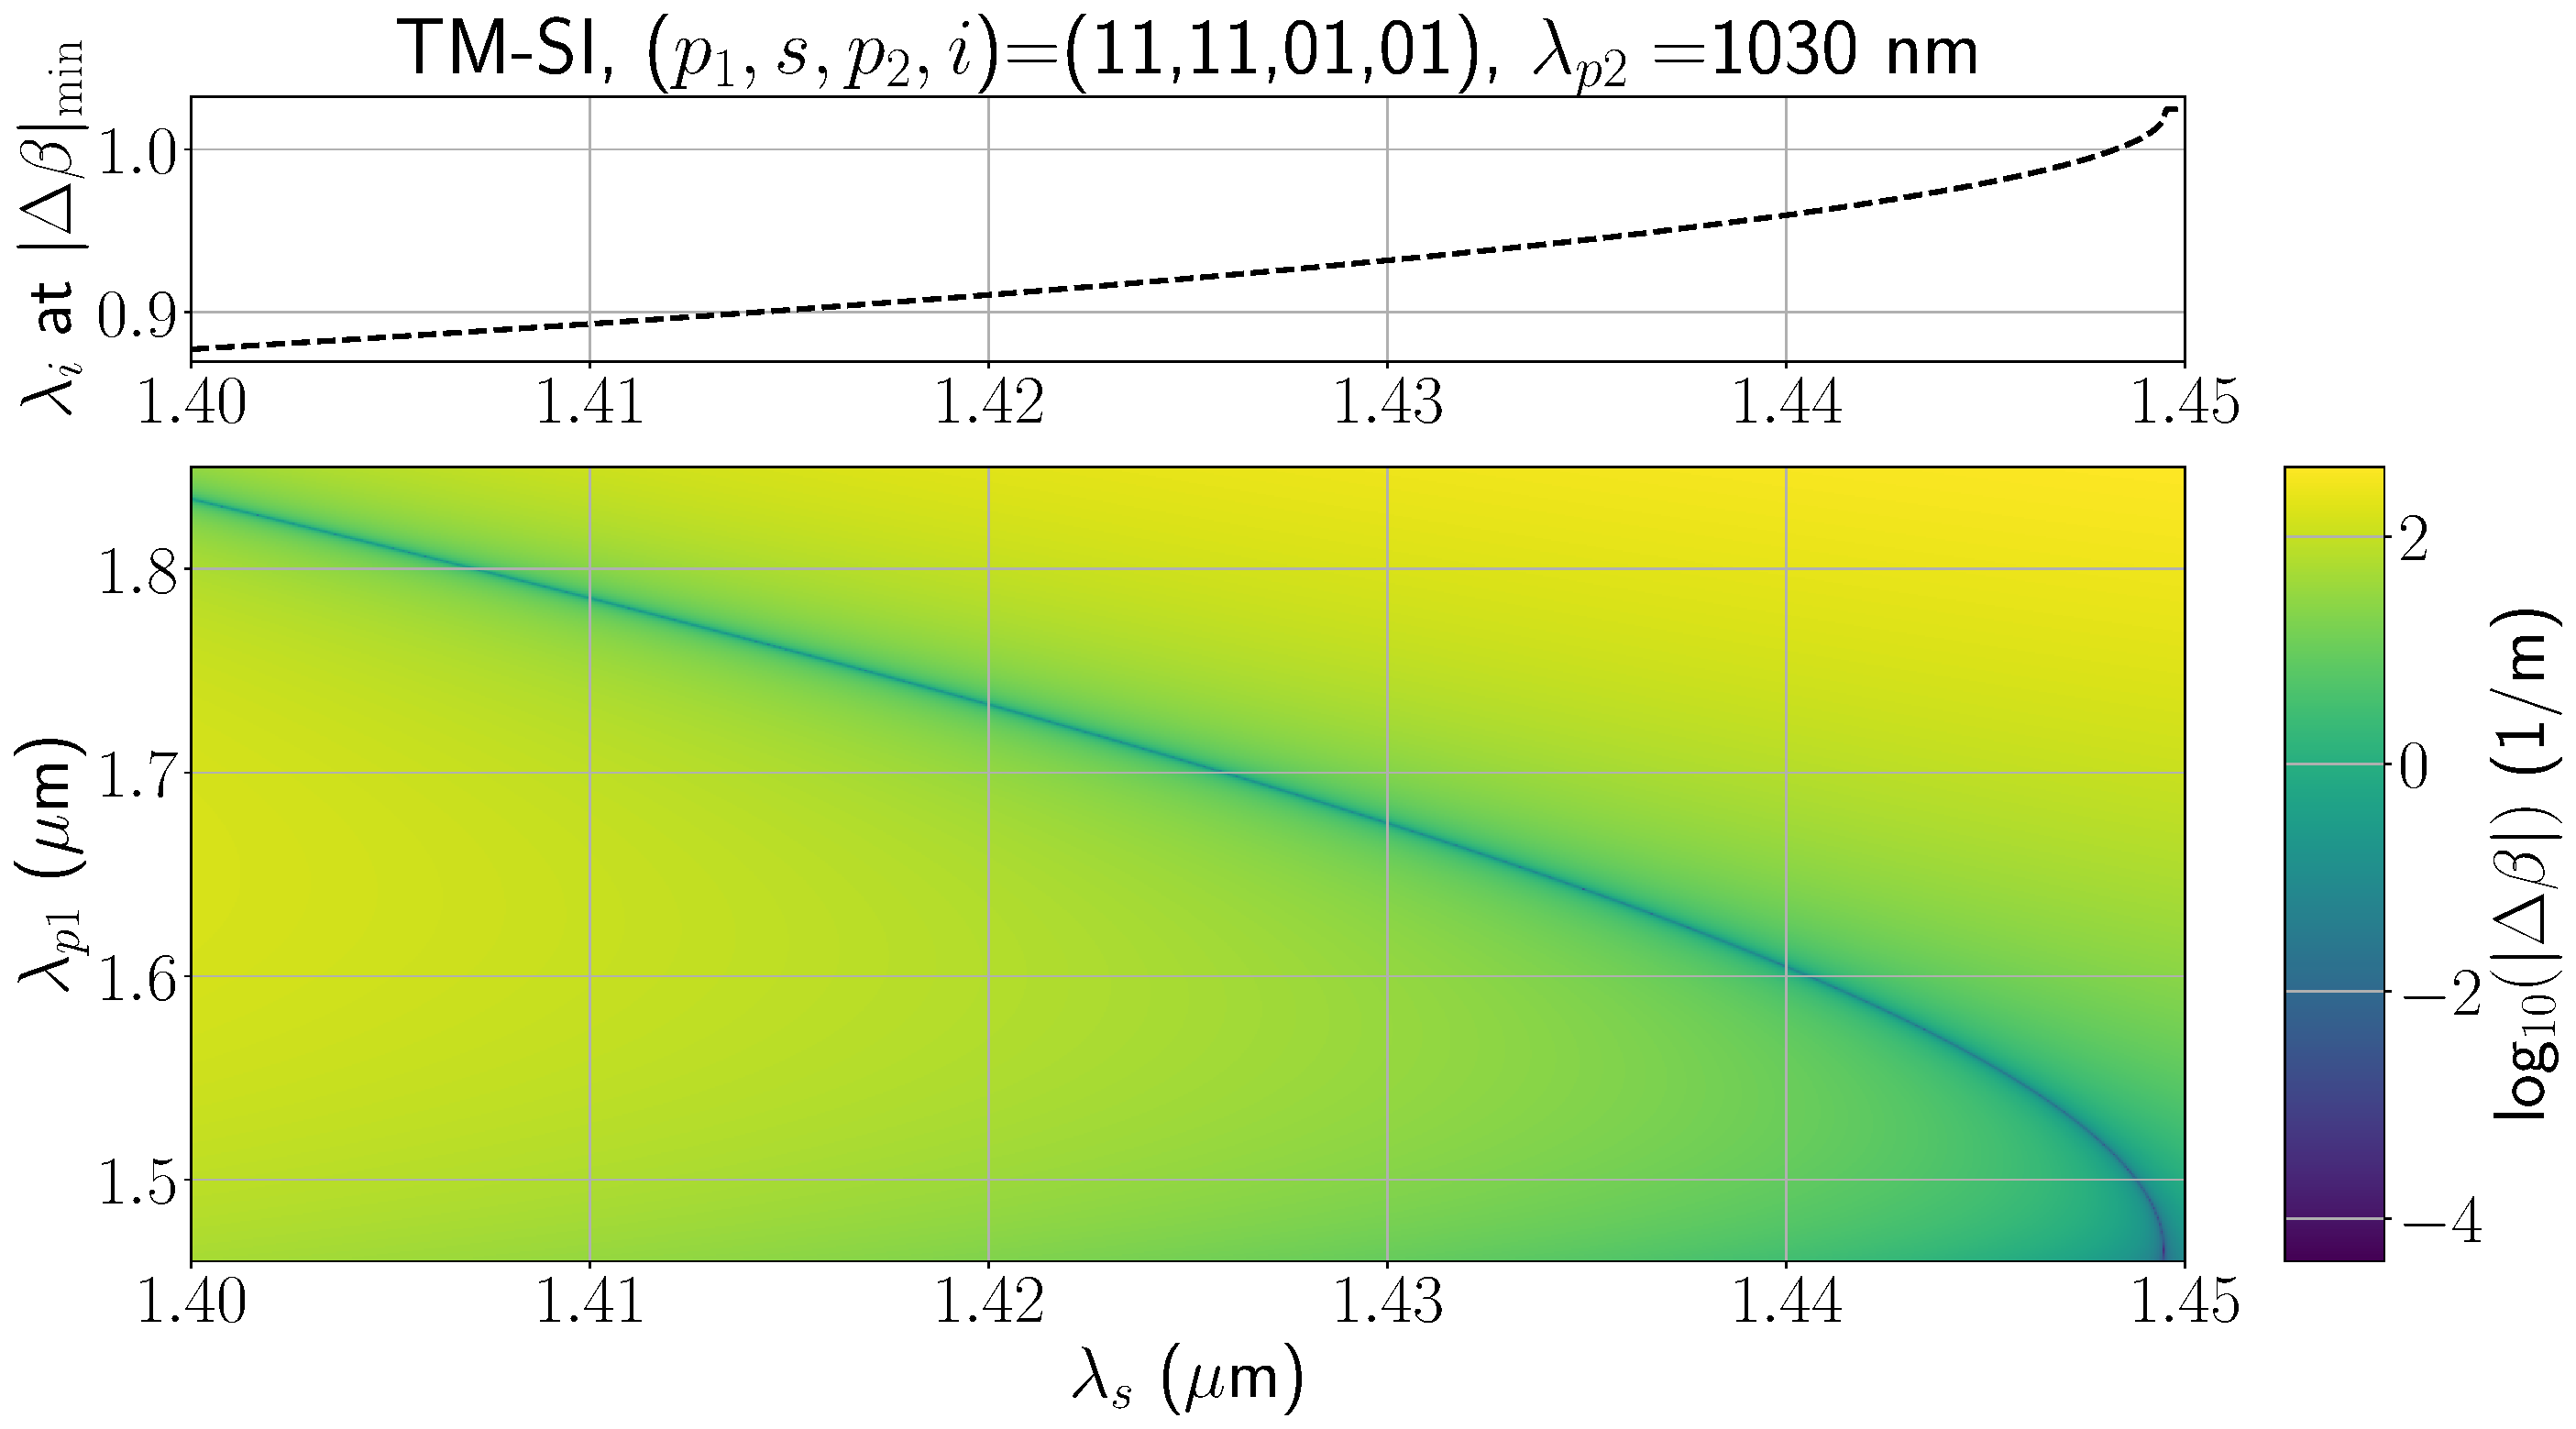
\includegraphics[width=0.8\textwidth]{./figs/TMSI_(11,11,01,01)_1030_2d_dbeta.pdf}
    \caption{}
    \label{fig:hom_1030}
\end{figure}
\subsubsection*{Setups}
$\lambda_s=950,\lambda_{p2}=1030,\lambda_i=1440,\lambda_{\mathrm{p1}}=1600$. If using 1030 as SPS, single photons will be at $\sim$ 940 nm, hopefully we can find phase matching while staying within L-band (can be tested classically).
\begin{figure}[h]
\begin{minipage}[t]{0.5\textwidth}
    \textbf{Pros}
    \begin{itemize}
        \item Known setup
        \item Can be tested classically
        \item Very high pump power
    \end{itemize}
\end{minipage}%
\hfill
\begin{minipage}[t]{0.5\textwidth}
    \textbf{Cons}
    \begin{itemize}
        \item Walk-off (can be reduced if using Aeropulse)
        \item Clocking C/L with 1030/SPS
        \item Phase matching possible while staying within L-band?
    \end{itemize}
\end{minipage}
\end{figure}
\newpage
\begin{figure}[h]
    \centering
    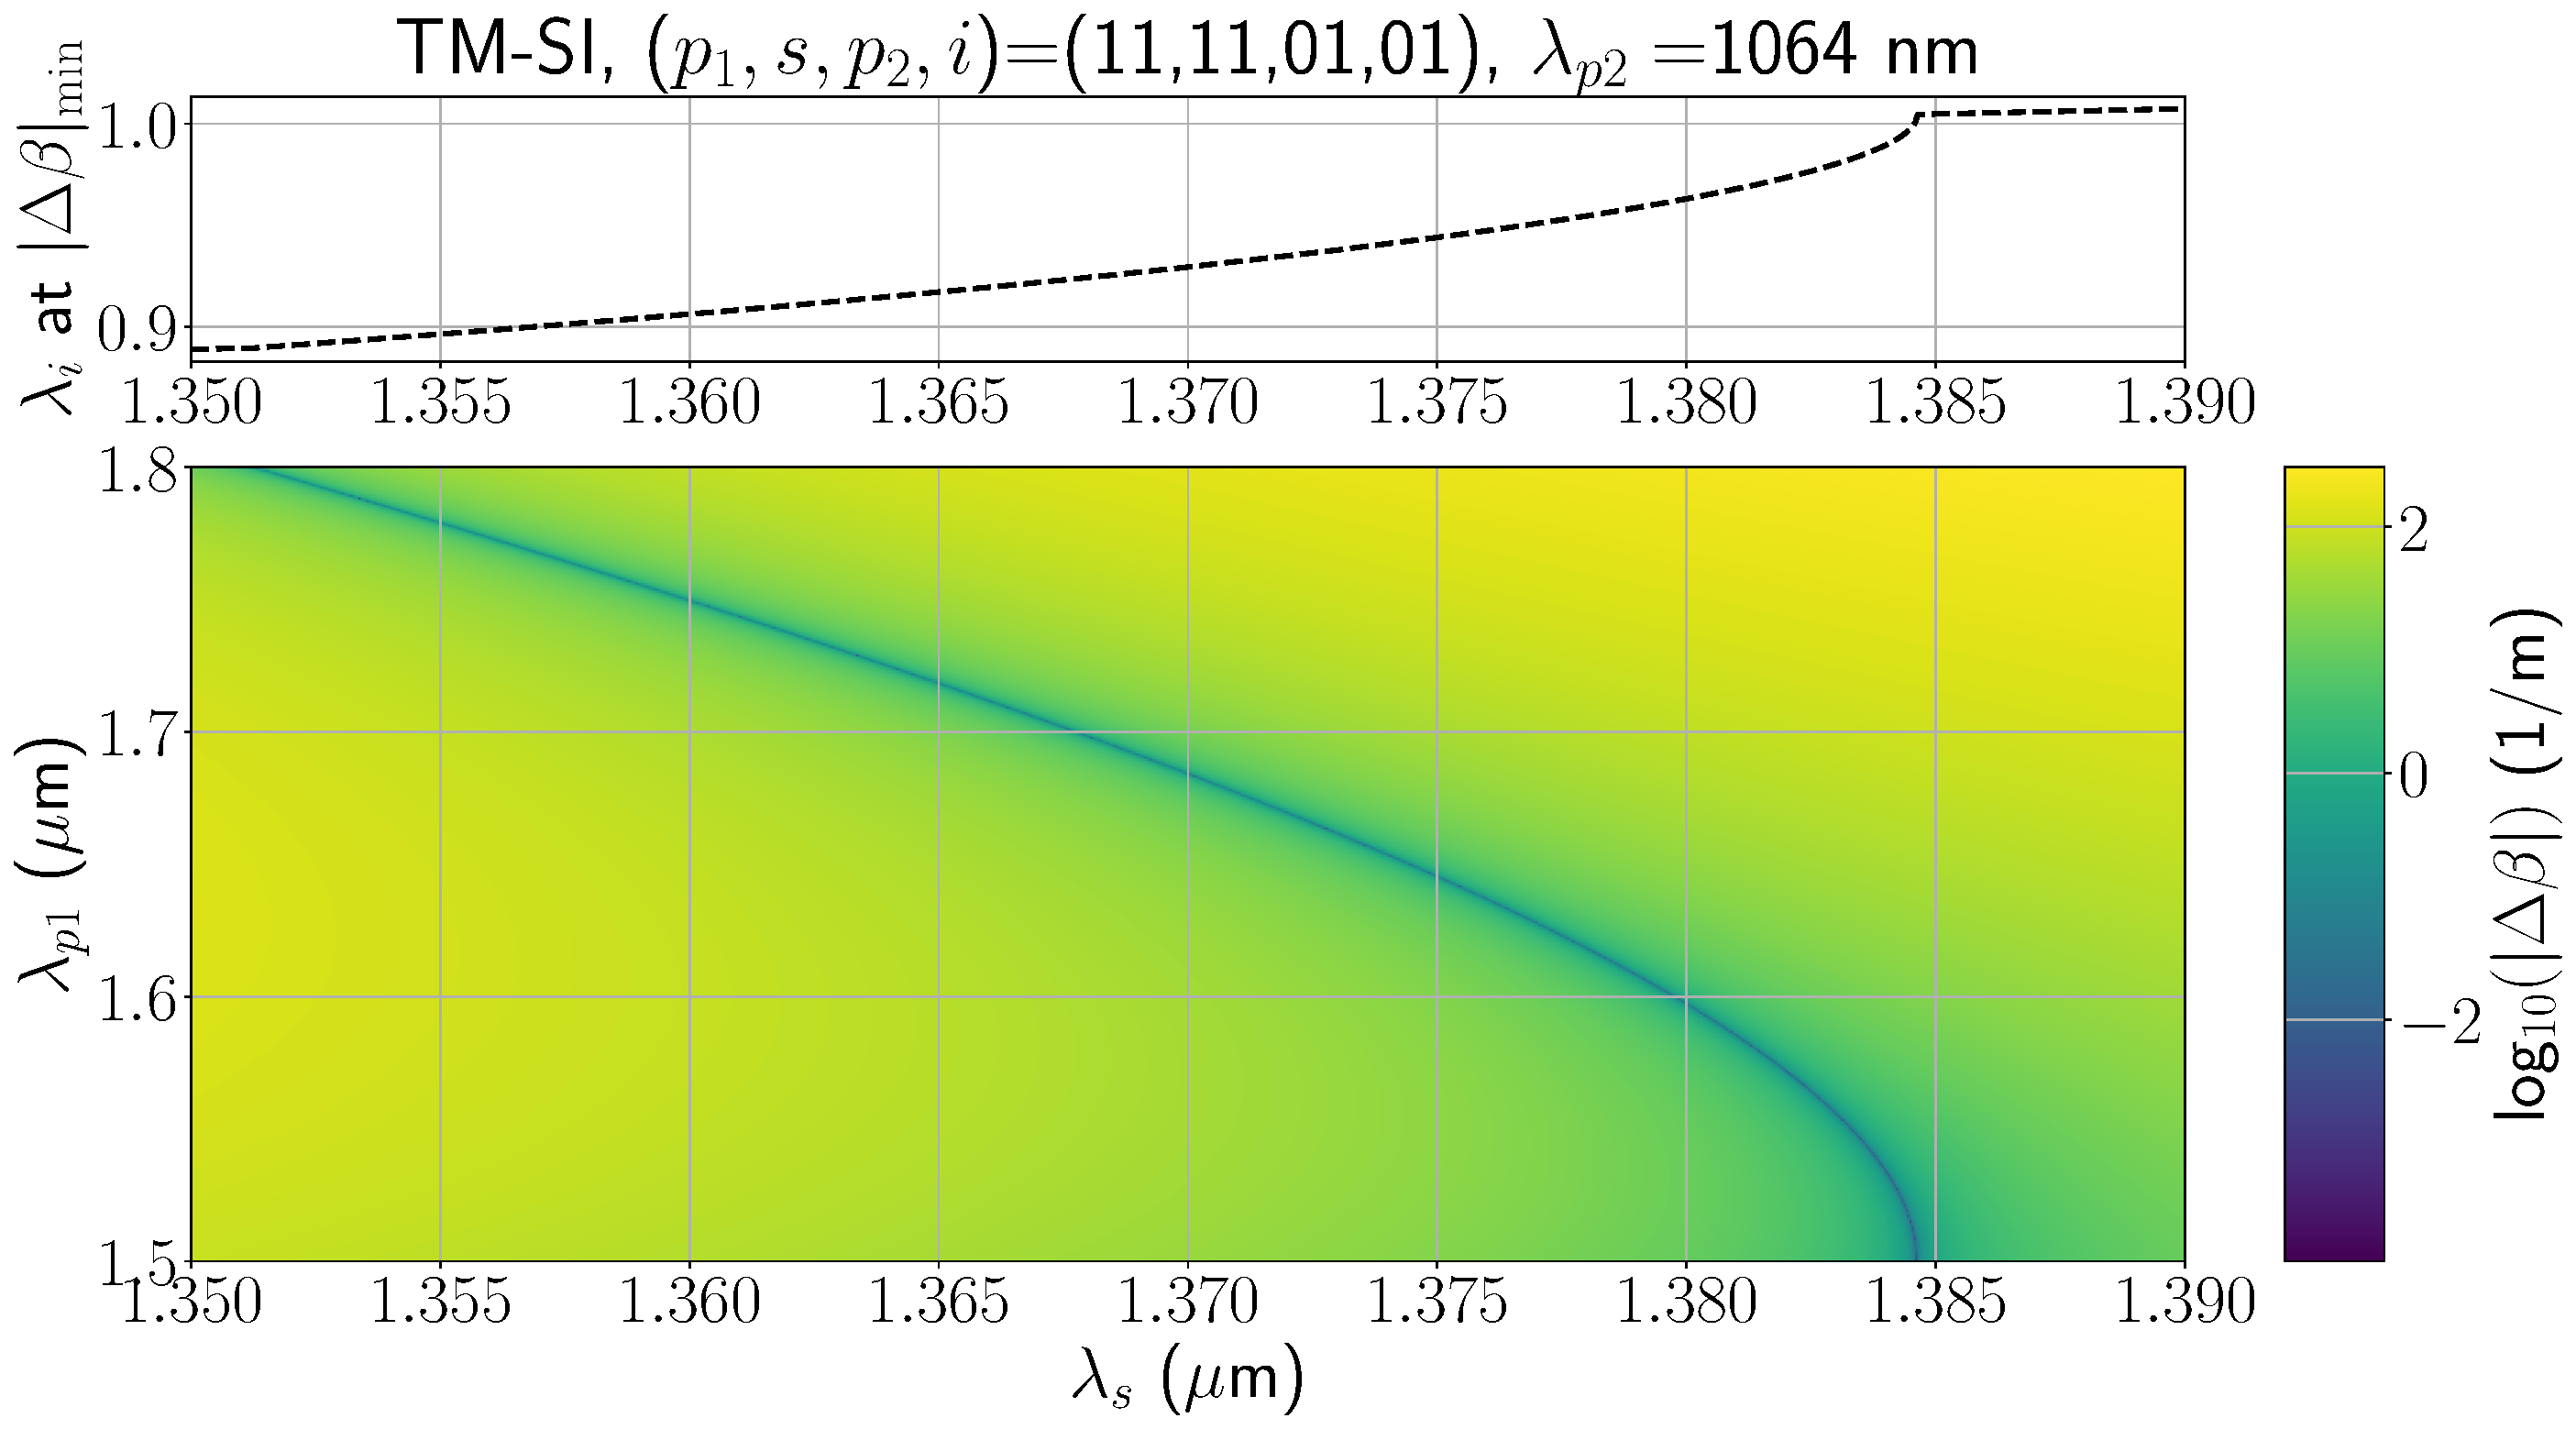
\includegraphics[width=0.8\textwidth]{./figs/TMSI_(11,11,01,01)_1064_2d_dbeta.pdf}
    \caption{}
    \label{fig:hom_1064}
\end{figure}
$\lambda_s=950,\lambda_{p2}=1064,\lambda_i=1380,\lambda_{\mathrm{p1}}=1600$. If using 1064 as SPS, single photons will be at $\sim$ 965 nm, hopefully we can find phase matching while staying within L-band (can be tested classically).
\begin{figure}[h]
\begin{minipage}[t]{0.5\textwidth}
    \textbf{Pros}
    \begin{itemize}
        \item Known setup
        \item Can be tested classically
        \item High pump power
        \item Larger separation than with 1030 (maybe not necessary?)
    \end{itemize}
\end{minipage}%
\hfill
\begin{minipage}[t]{0.5\textwidth}
    \textbf{Cons}
    \begin{itemize}
        \item Walk-off (can be reduced if using Aeropulse)
        \item Clocking C/L with 1064/SPS
        \item Phase matching possible while staying within L-band?
    \end{itemize}
\end{minipage}
\end{figure}
\newpage
\subsubsection{Nearby BS of quantum states using C+L band pumps}
\begin{figure}[H]
    \centering
    \begin{minipage}{0.5\textwidth}
        \centering
        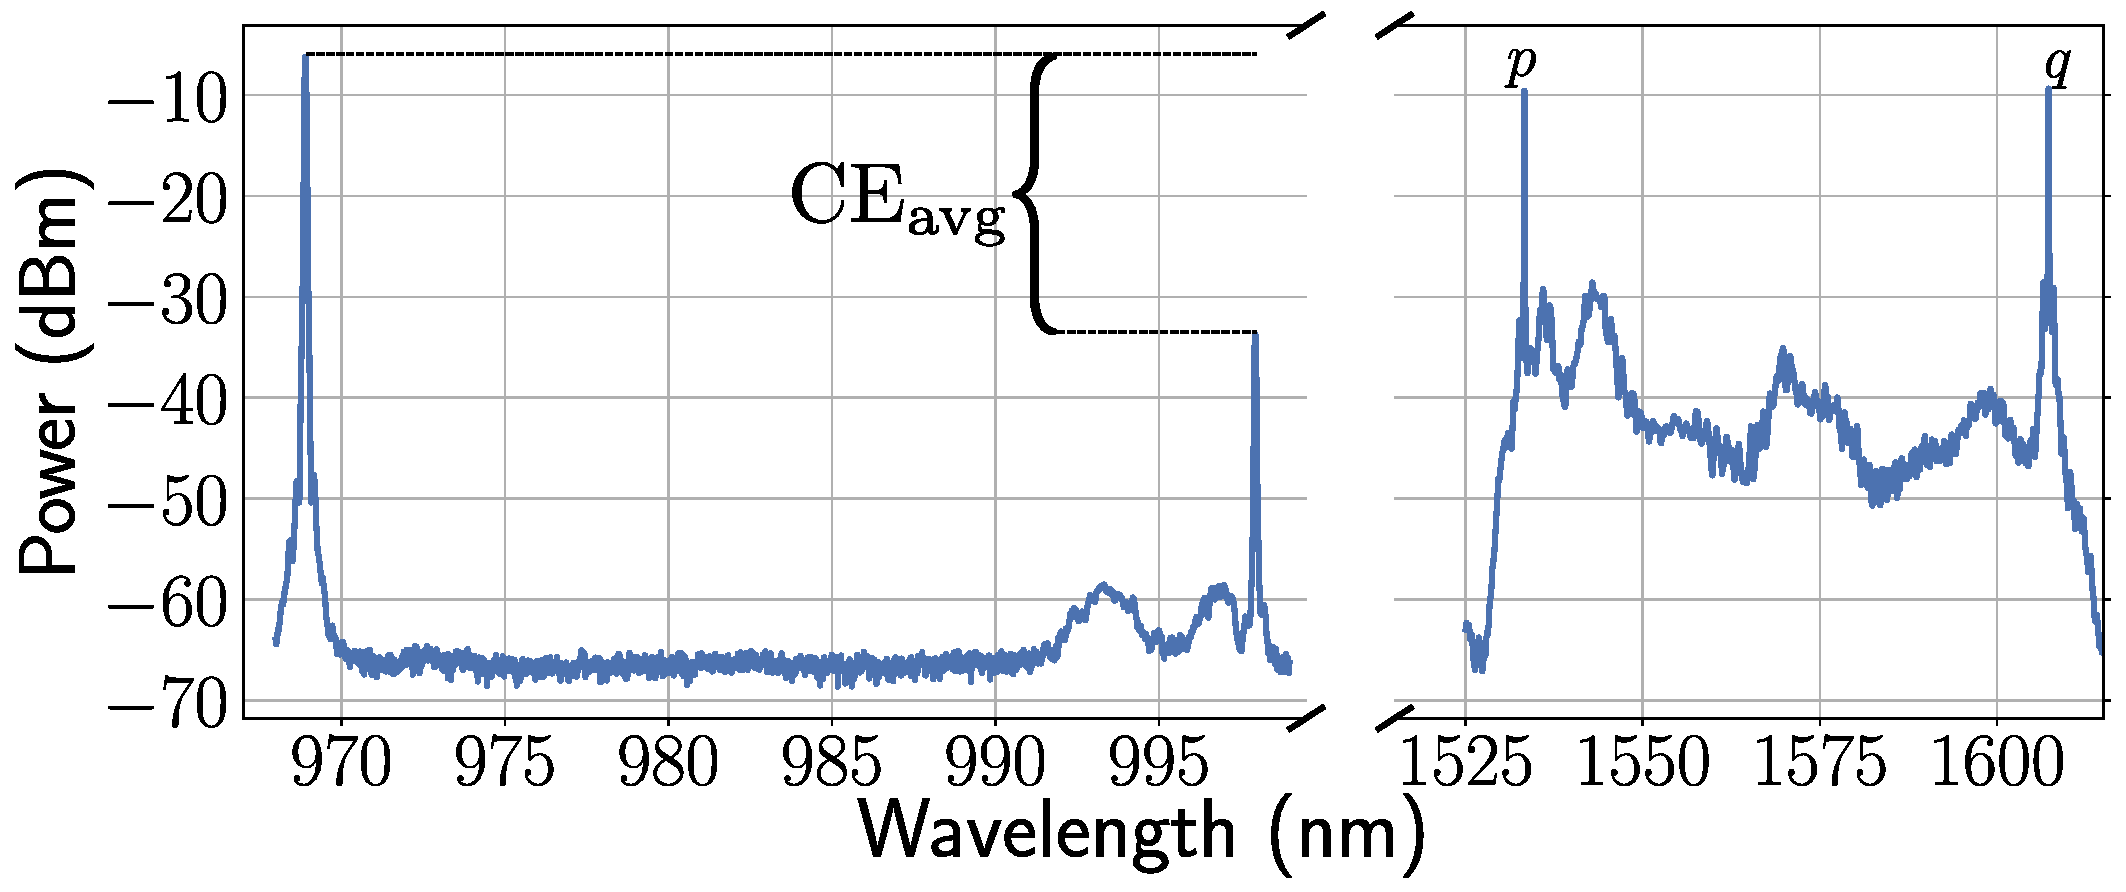
\includegraphics[width=\textwidth]{./figs/exp_data/spectra.pdf}
    \end{minipage}%
    \begin{minipage}{0.5\textwidth}
        \centering
        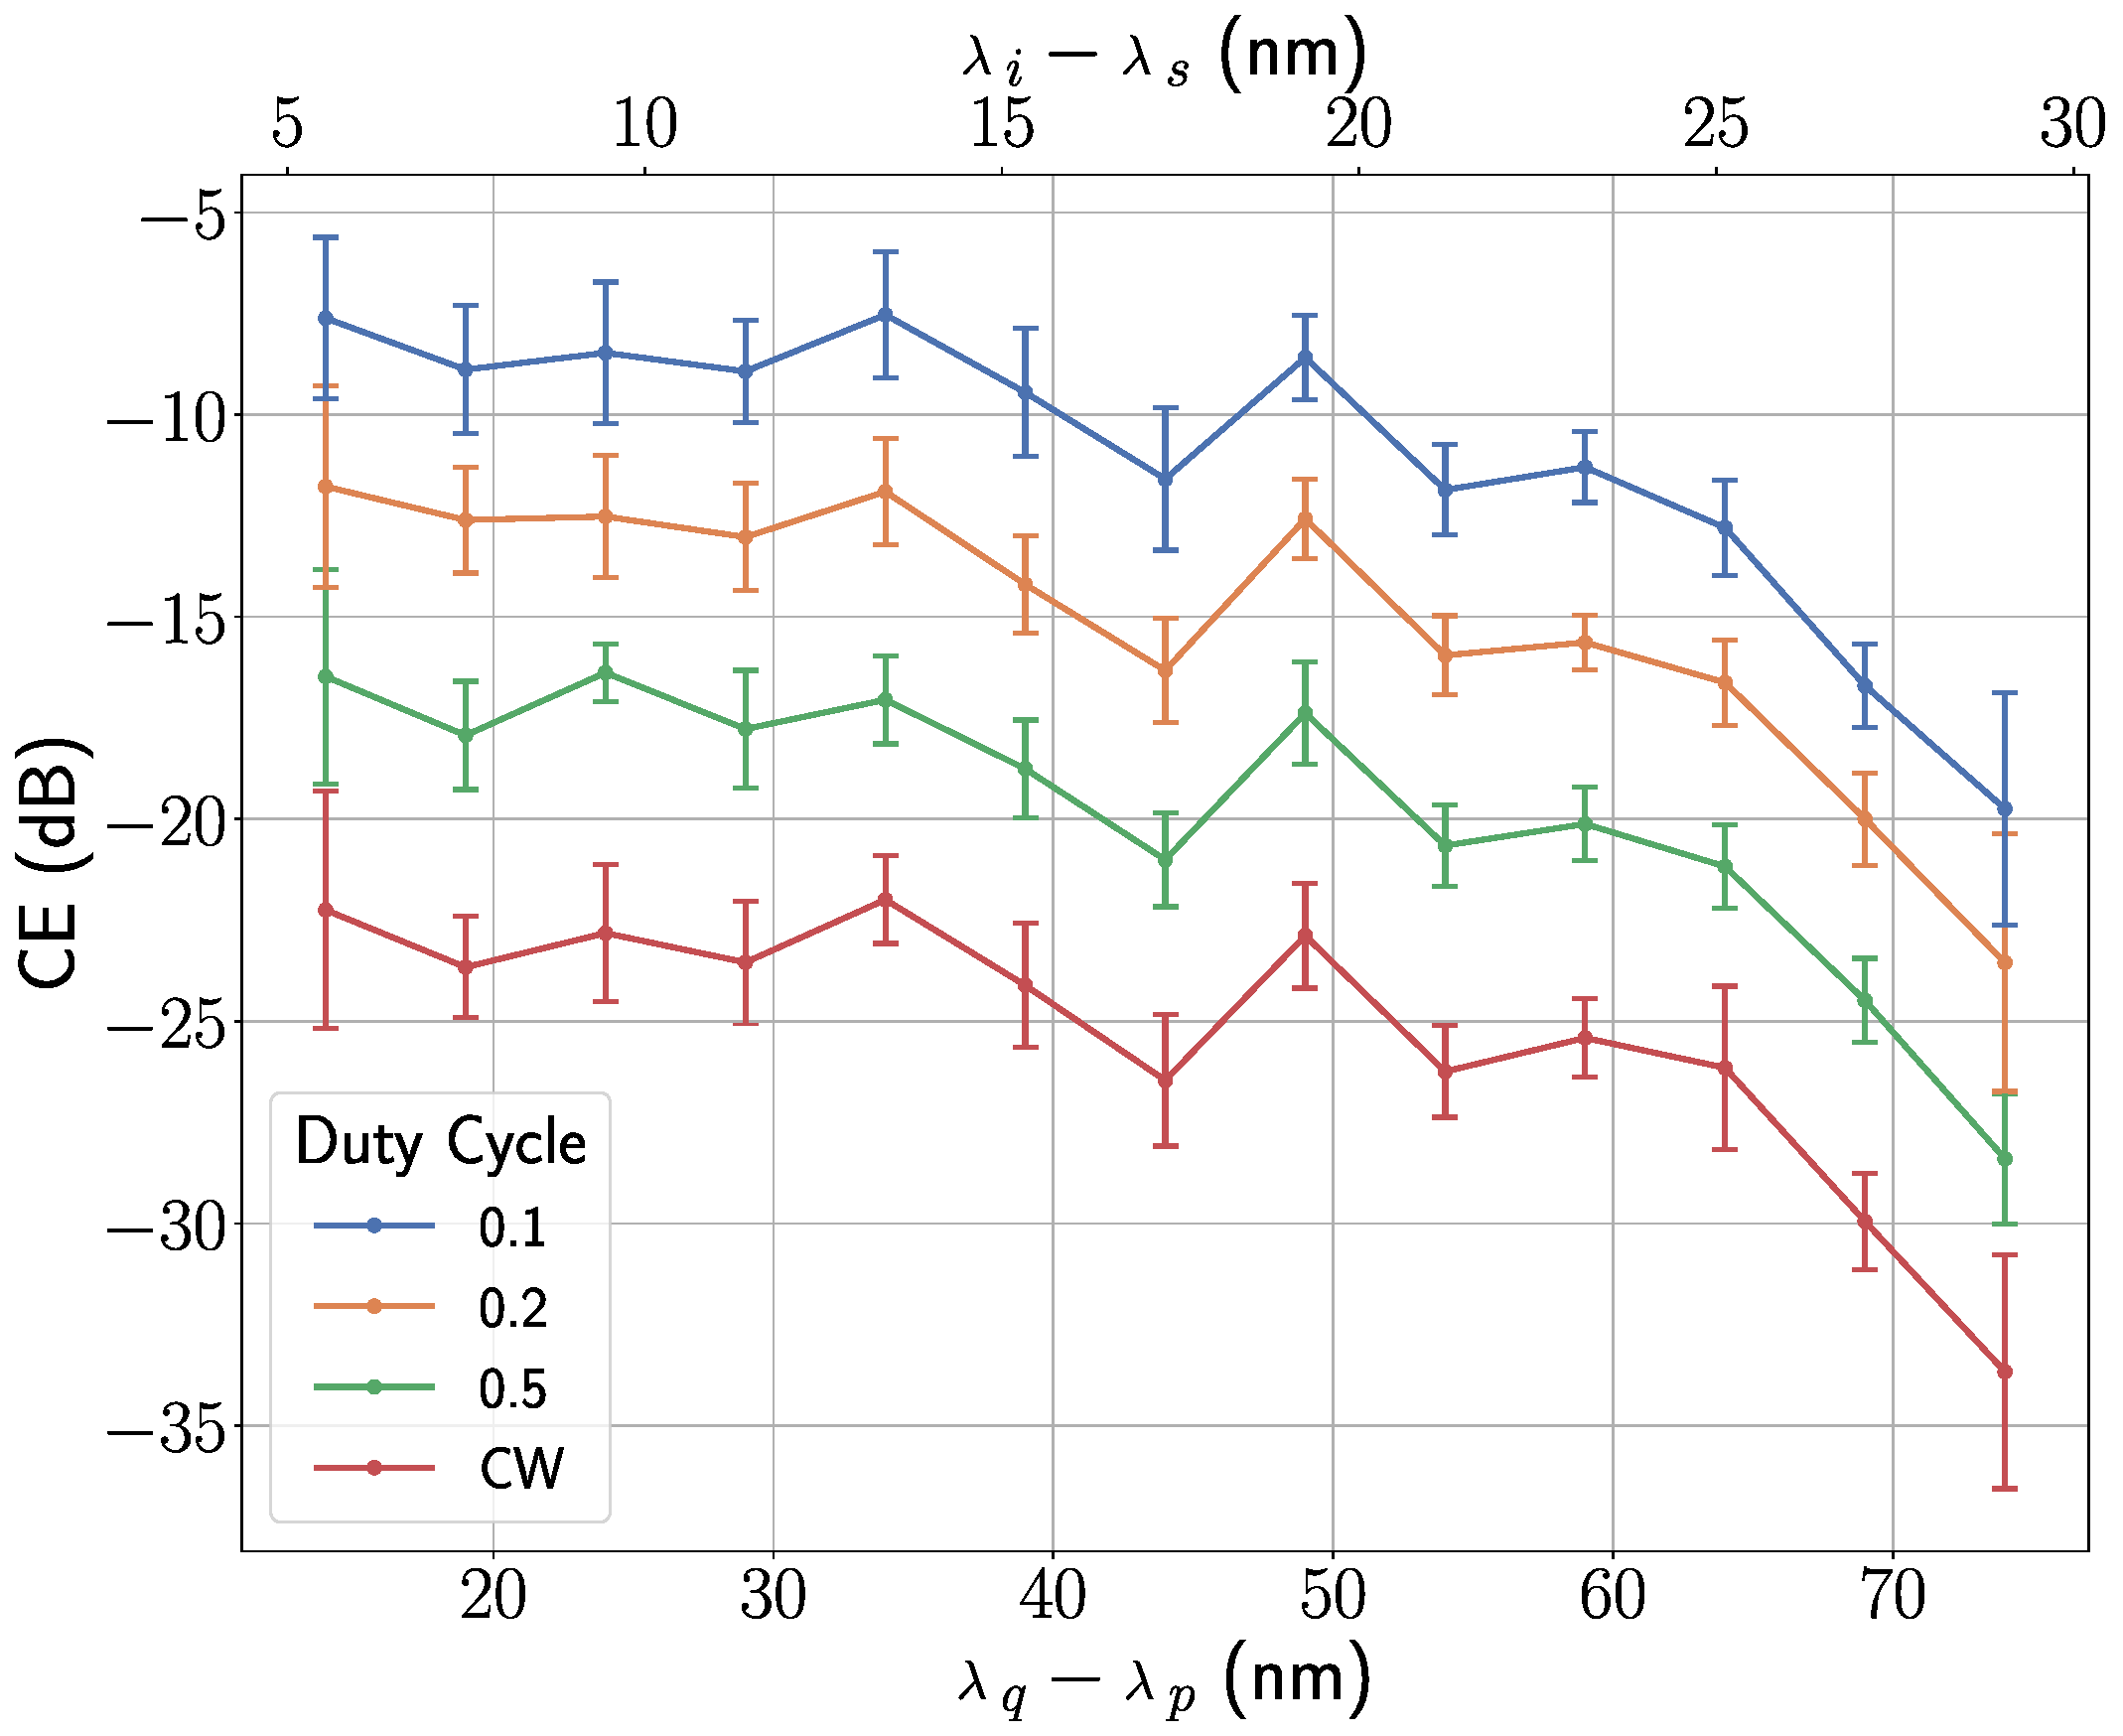
\includegraphics[width=\textwidth]{./figs/exp_data/ce_vs_pump_sep.pdf}
    \end{minipage}
    \caption{Exp data from cleo}
    \label{fig:exp_data}
\end{figure}
Initial test with FC of quantum states with nearby BS.

\newpage
\subsection{SMF, (01, 01, 01, 01)}
\begin{figure}[h]
    \centering
    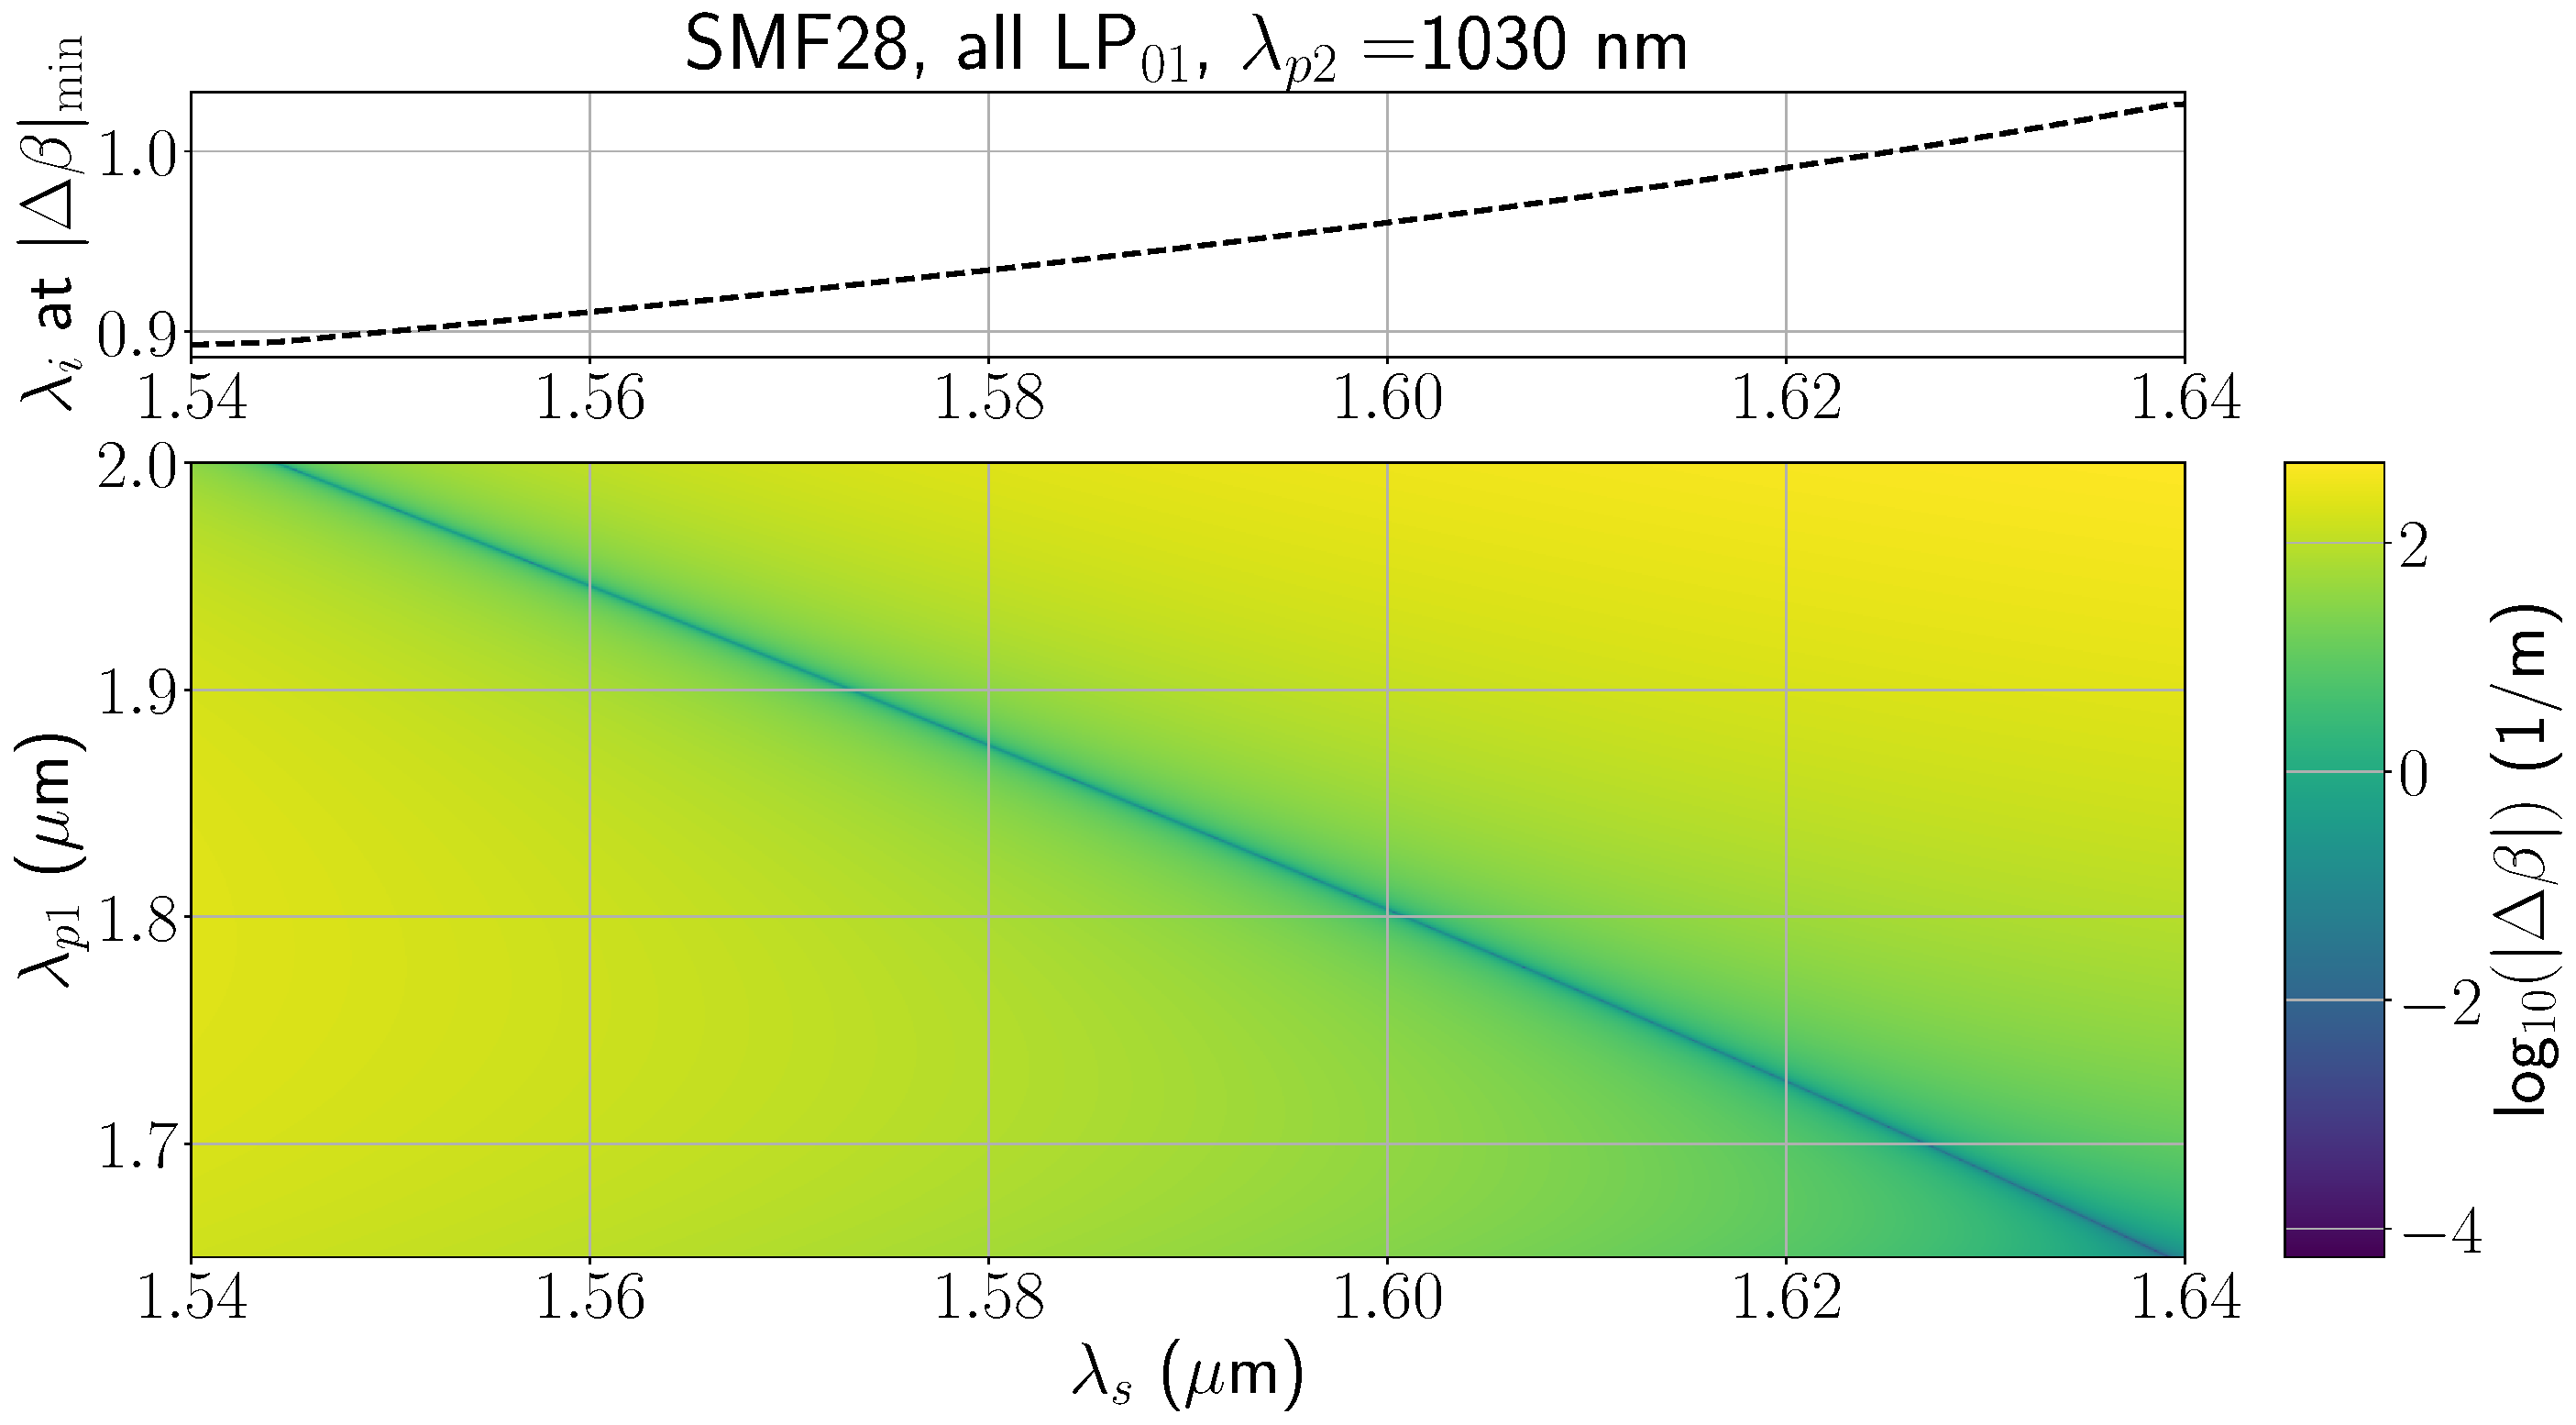
\includegraphics[width=0.8\textwidth]{./figs/SMF28_all_LP01_1030_2d_dbeta.pdf}
    \caption{}
    \label{fig:smf_1030}
\end{figure}
\begin{figure}[h]
    \centering
    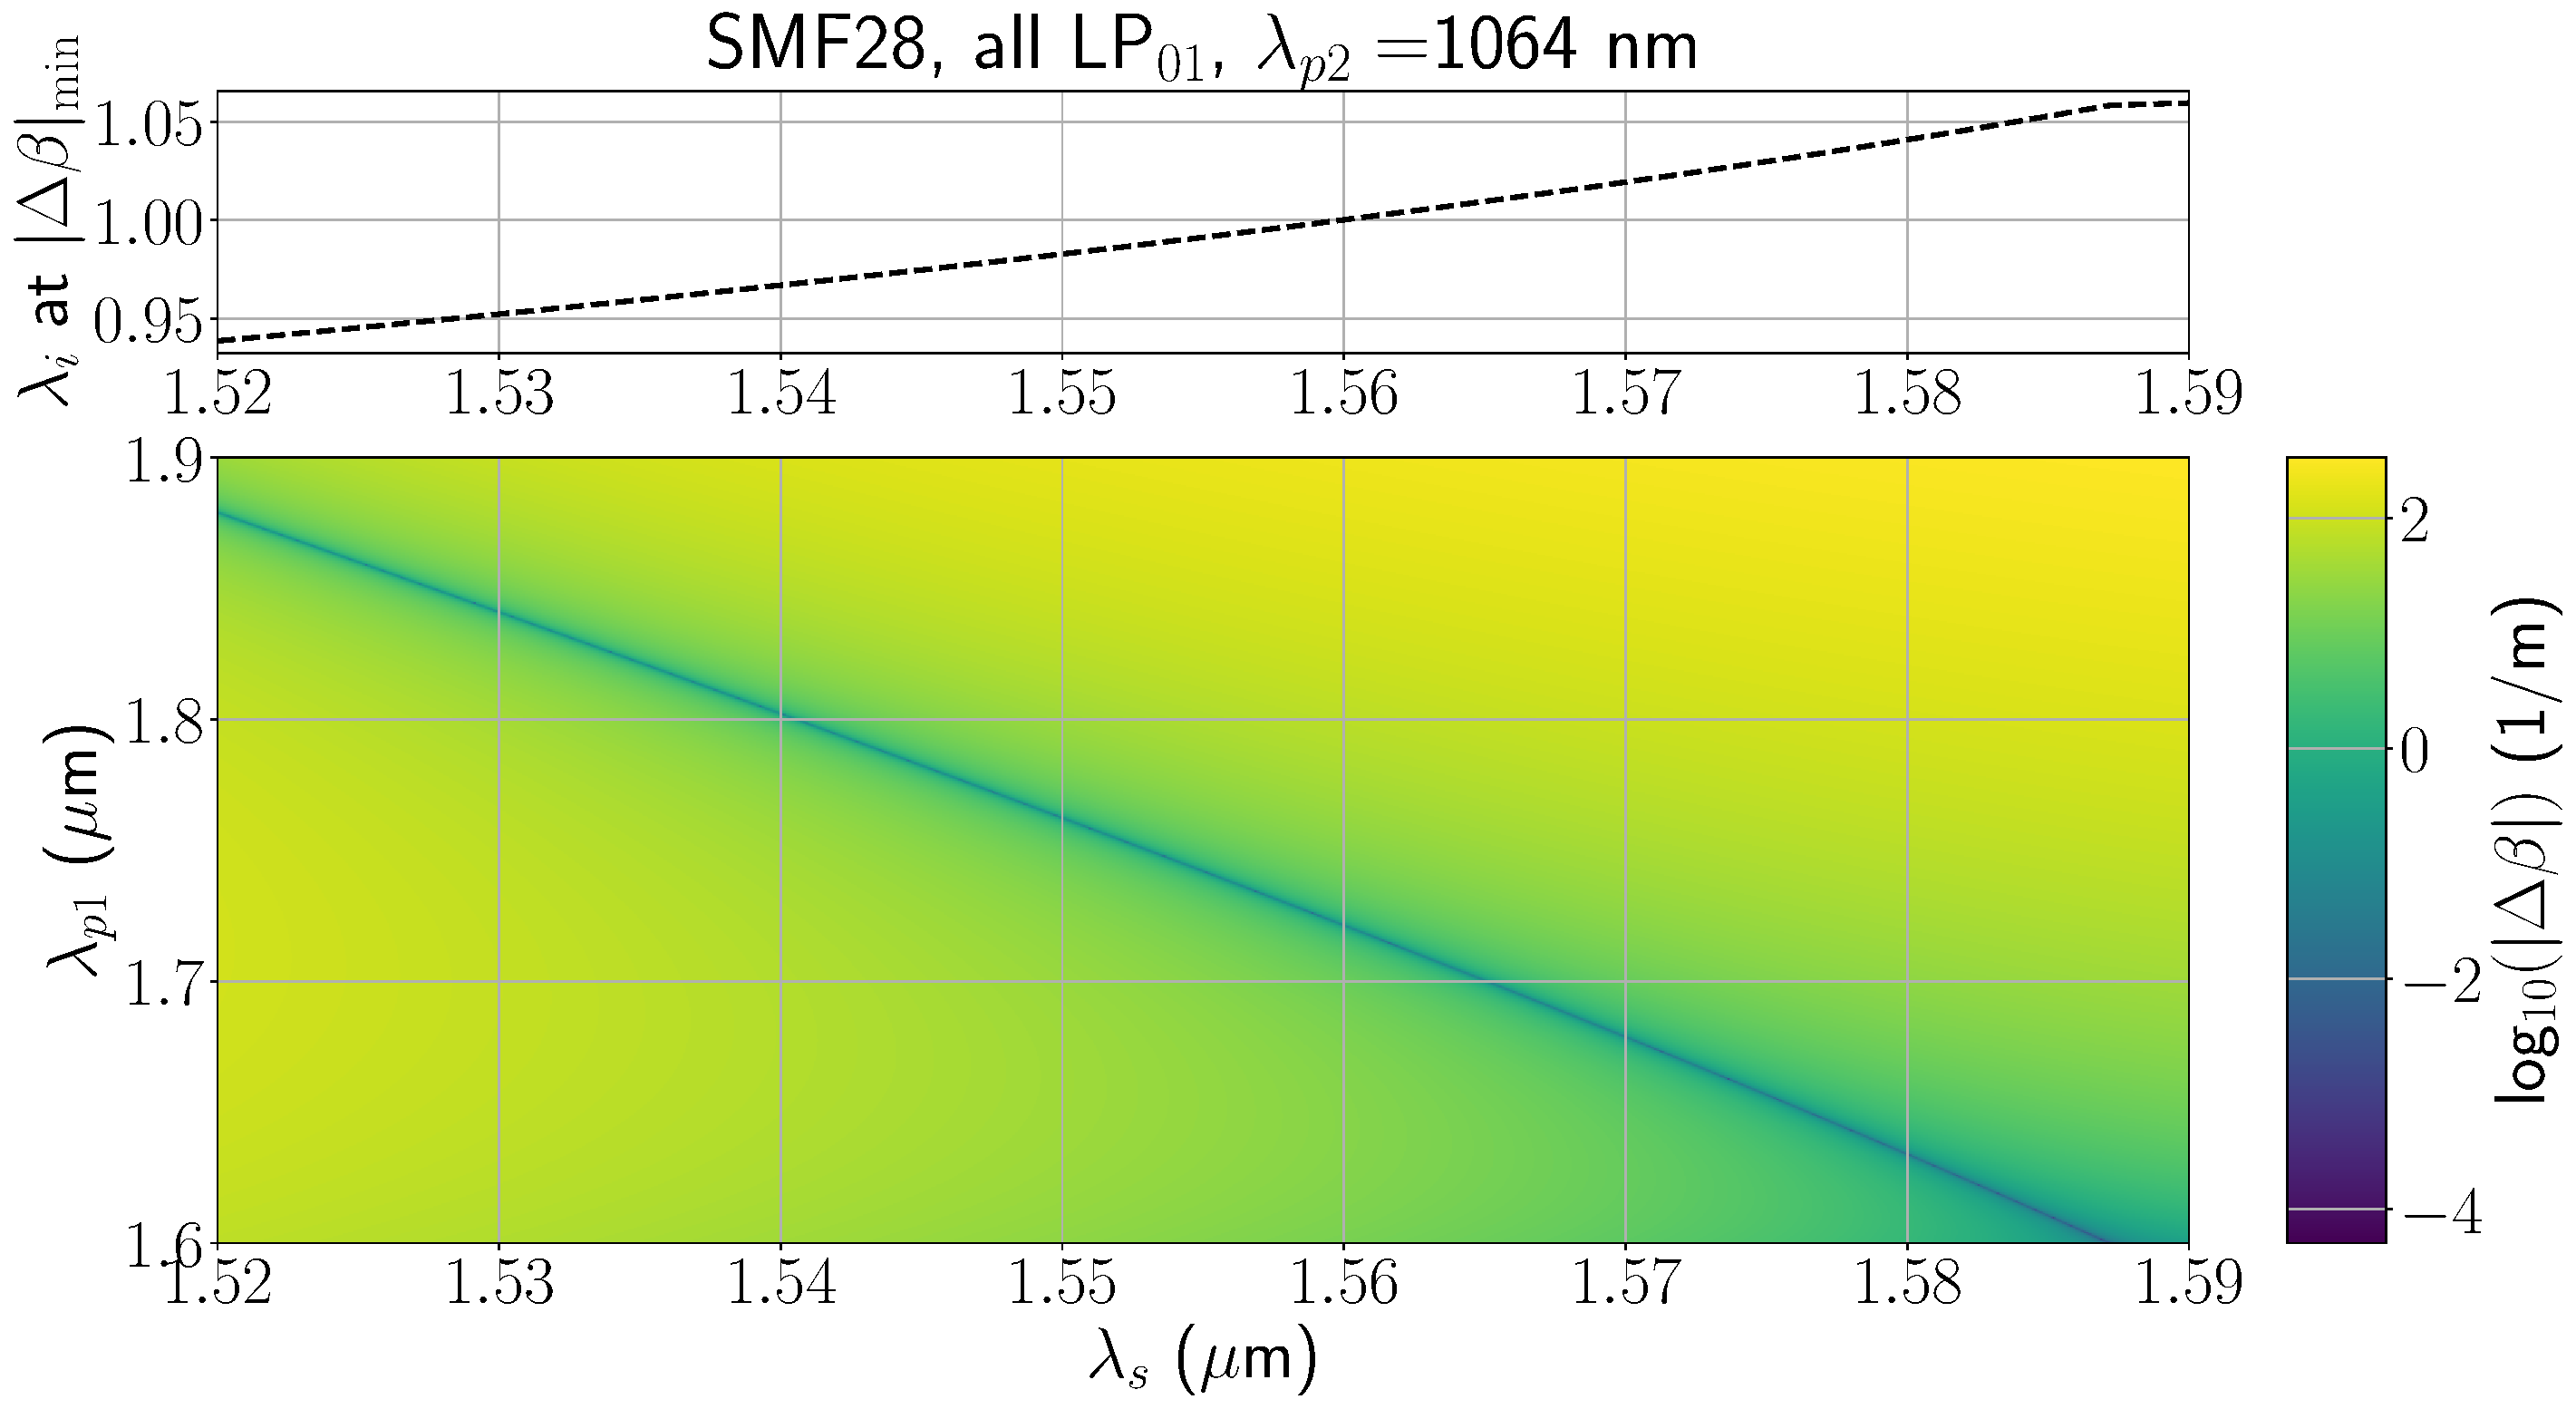
\includegraphics[width=0.8\textwidth]{./figs/SMF28_all_LP01_1064_2d_dbeta.pdf}
    \caption{}
    \label{fig:smf_1064}
\end{figure}
\newpage
\subsection{FMF, (01, 01, 01, 01)}
\begin{figure}[h]
    \centering
    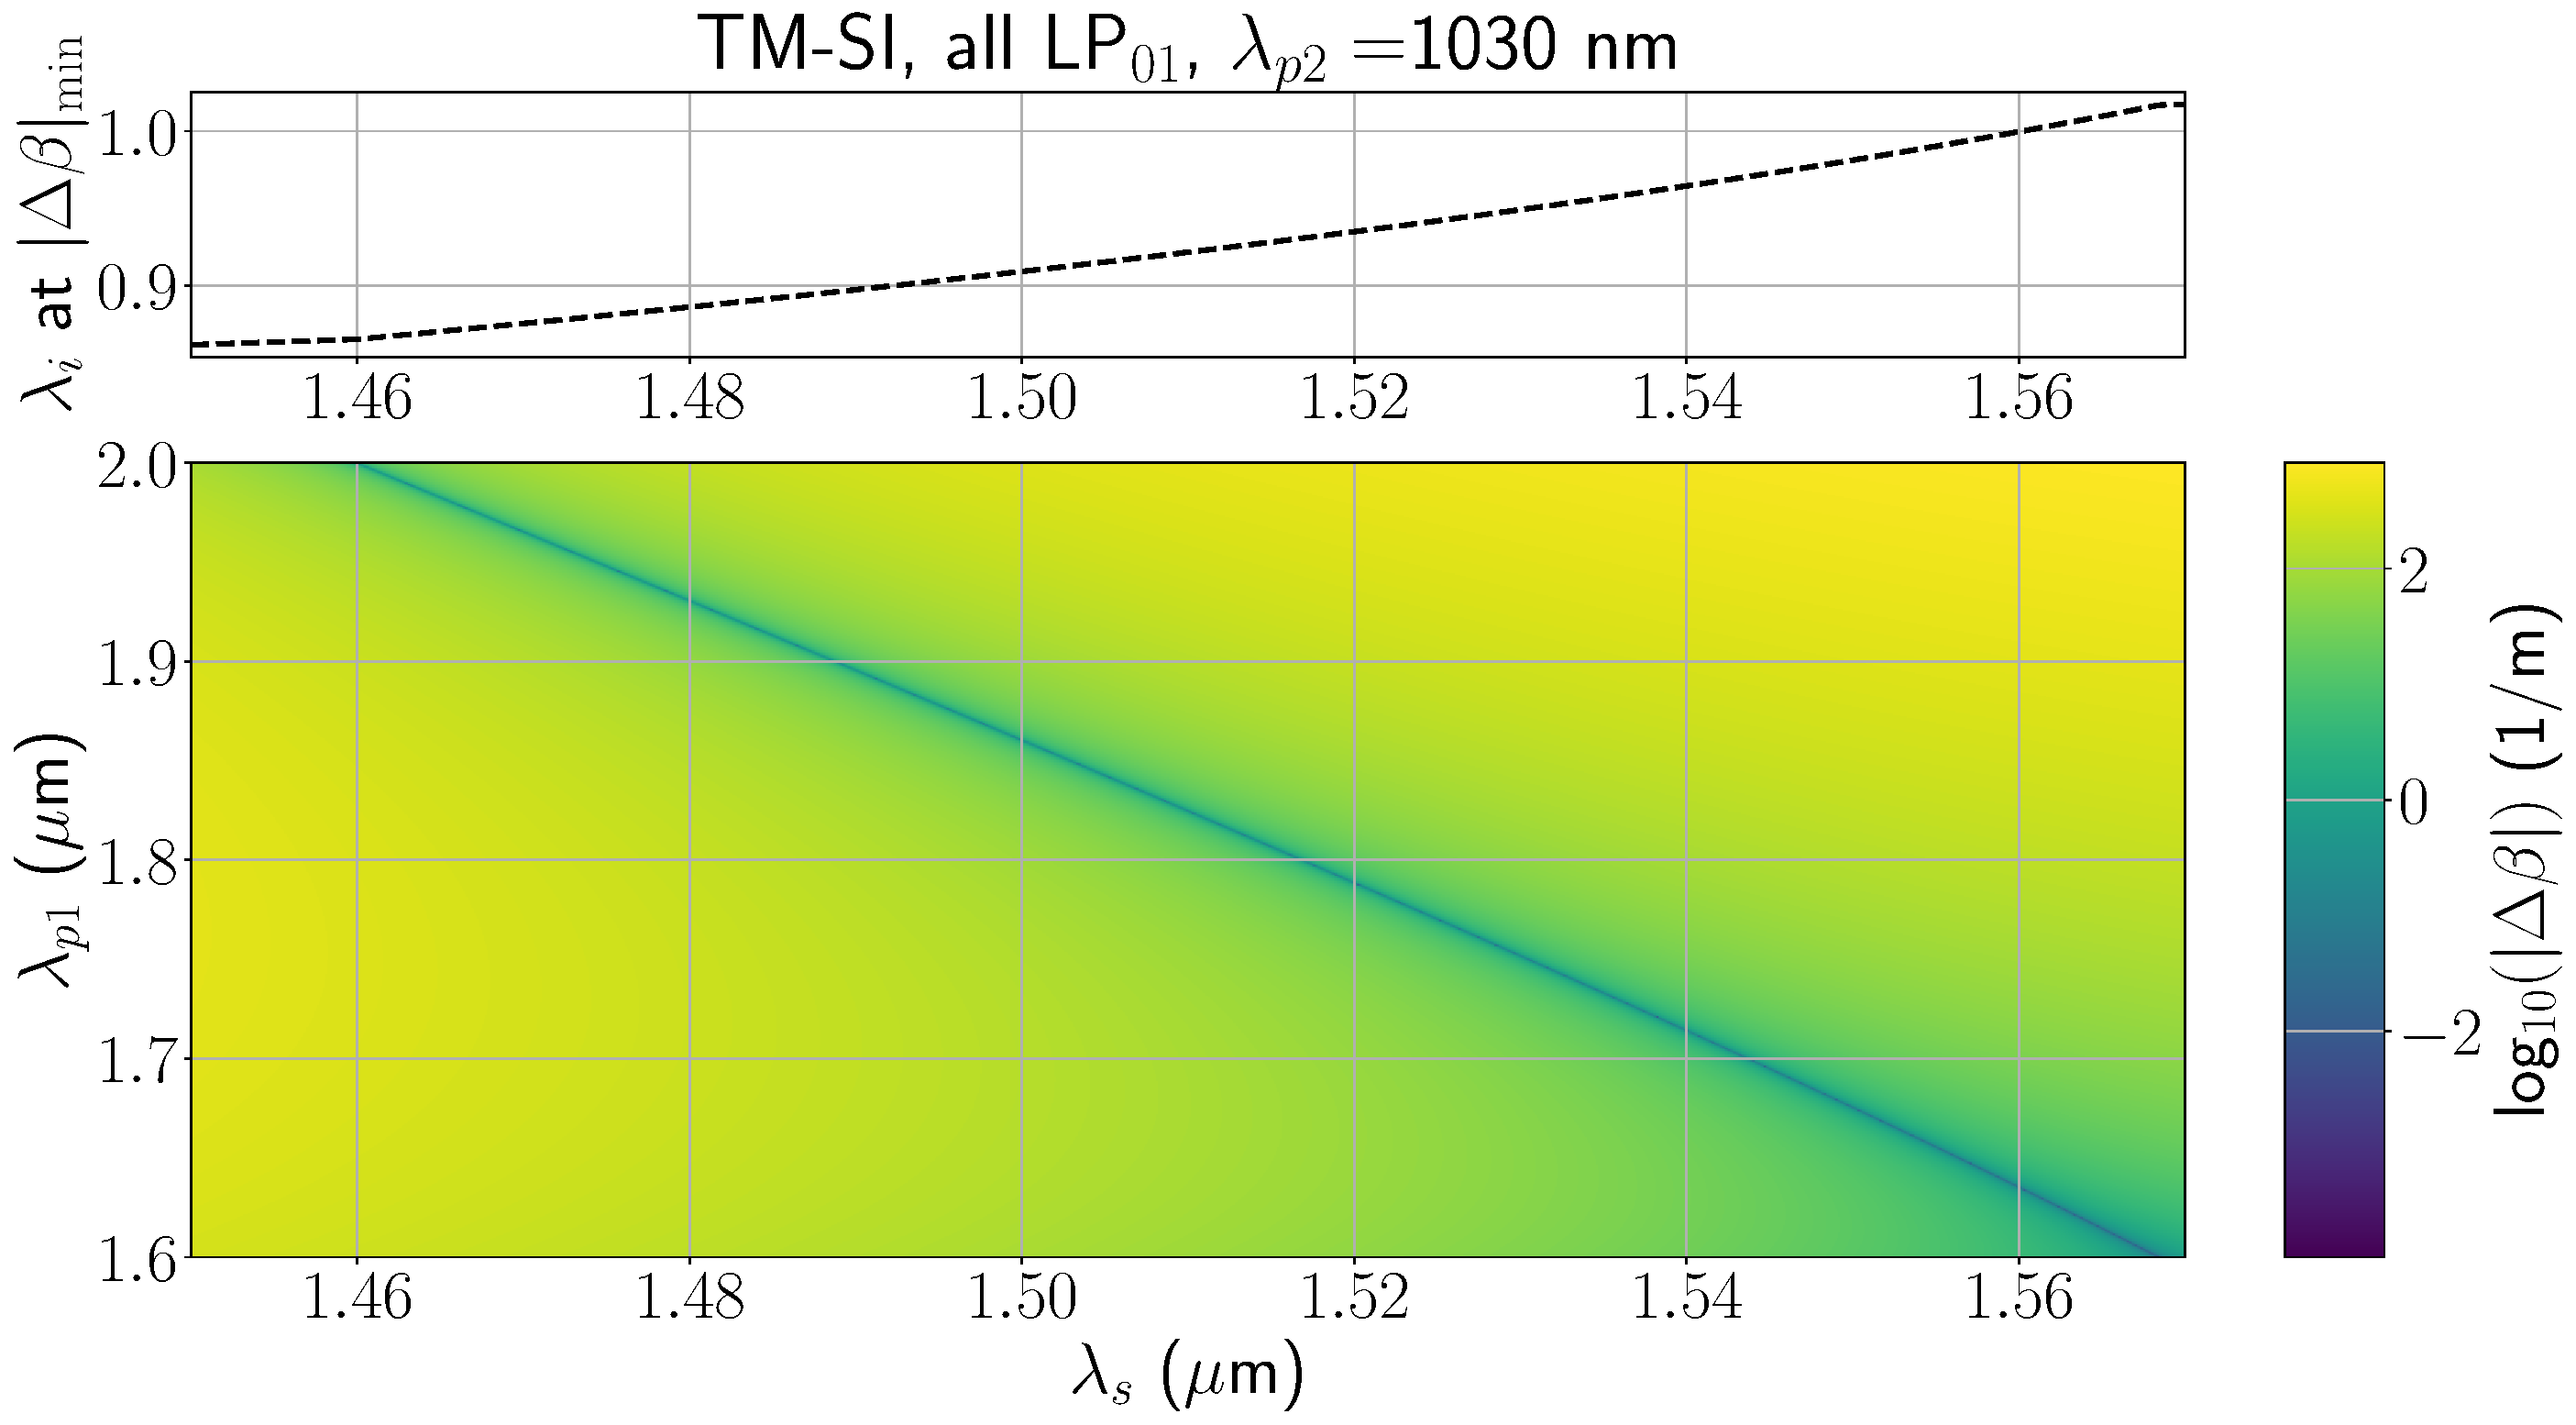
\includegraphics[width=0.8\textwidth]{./figs/TMSI_all_LP01_1030_2d_dbeta.pdf}
    \caption{}
    \label{fig:fmf_1030}
\end{figure}
\begin{figure}[h]
    \centering
    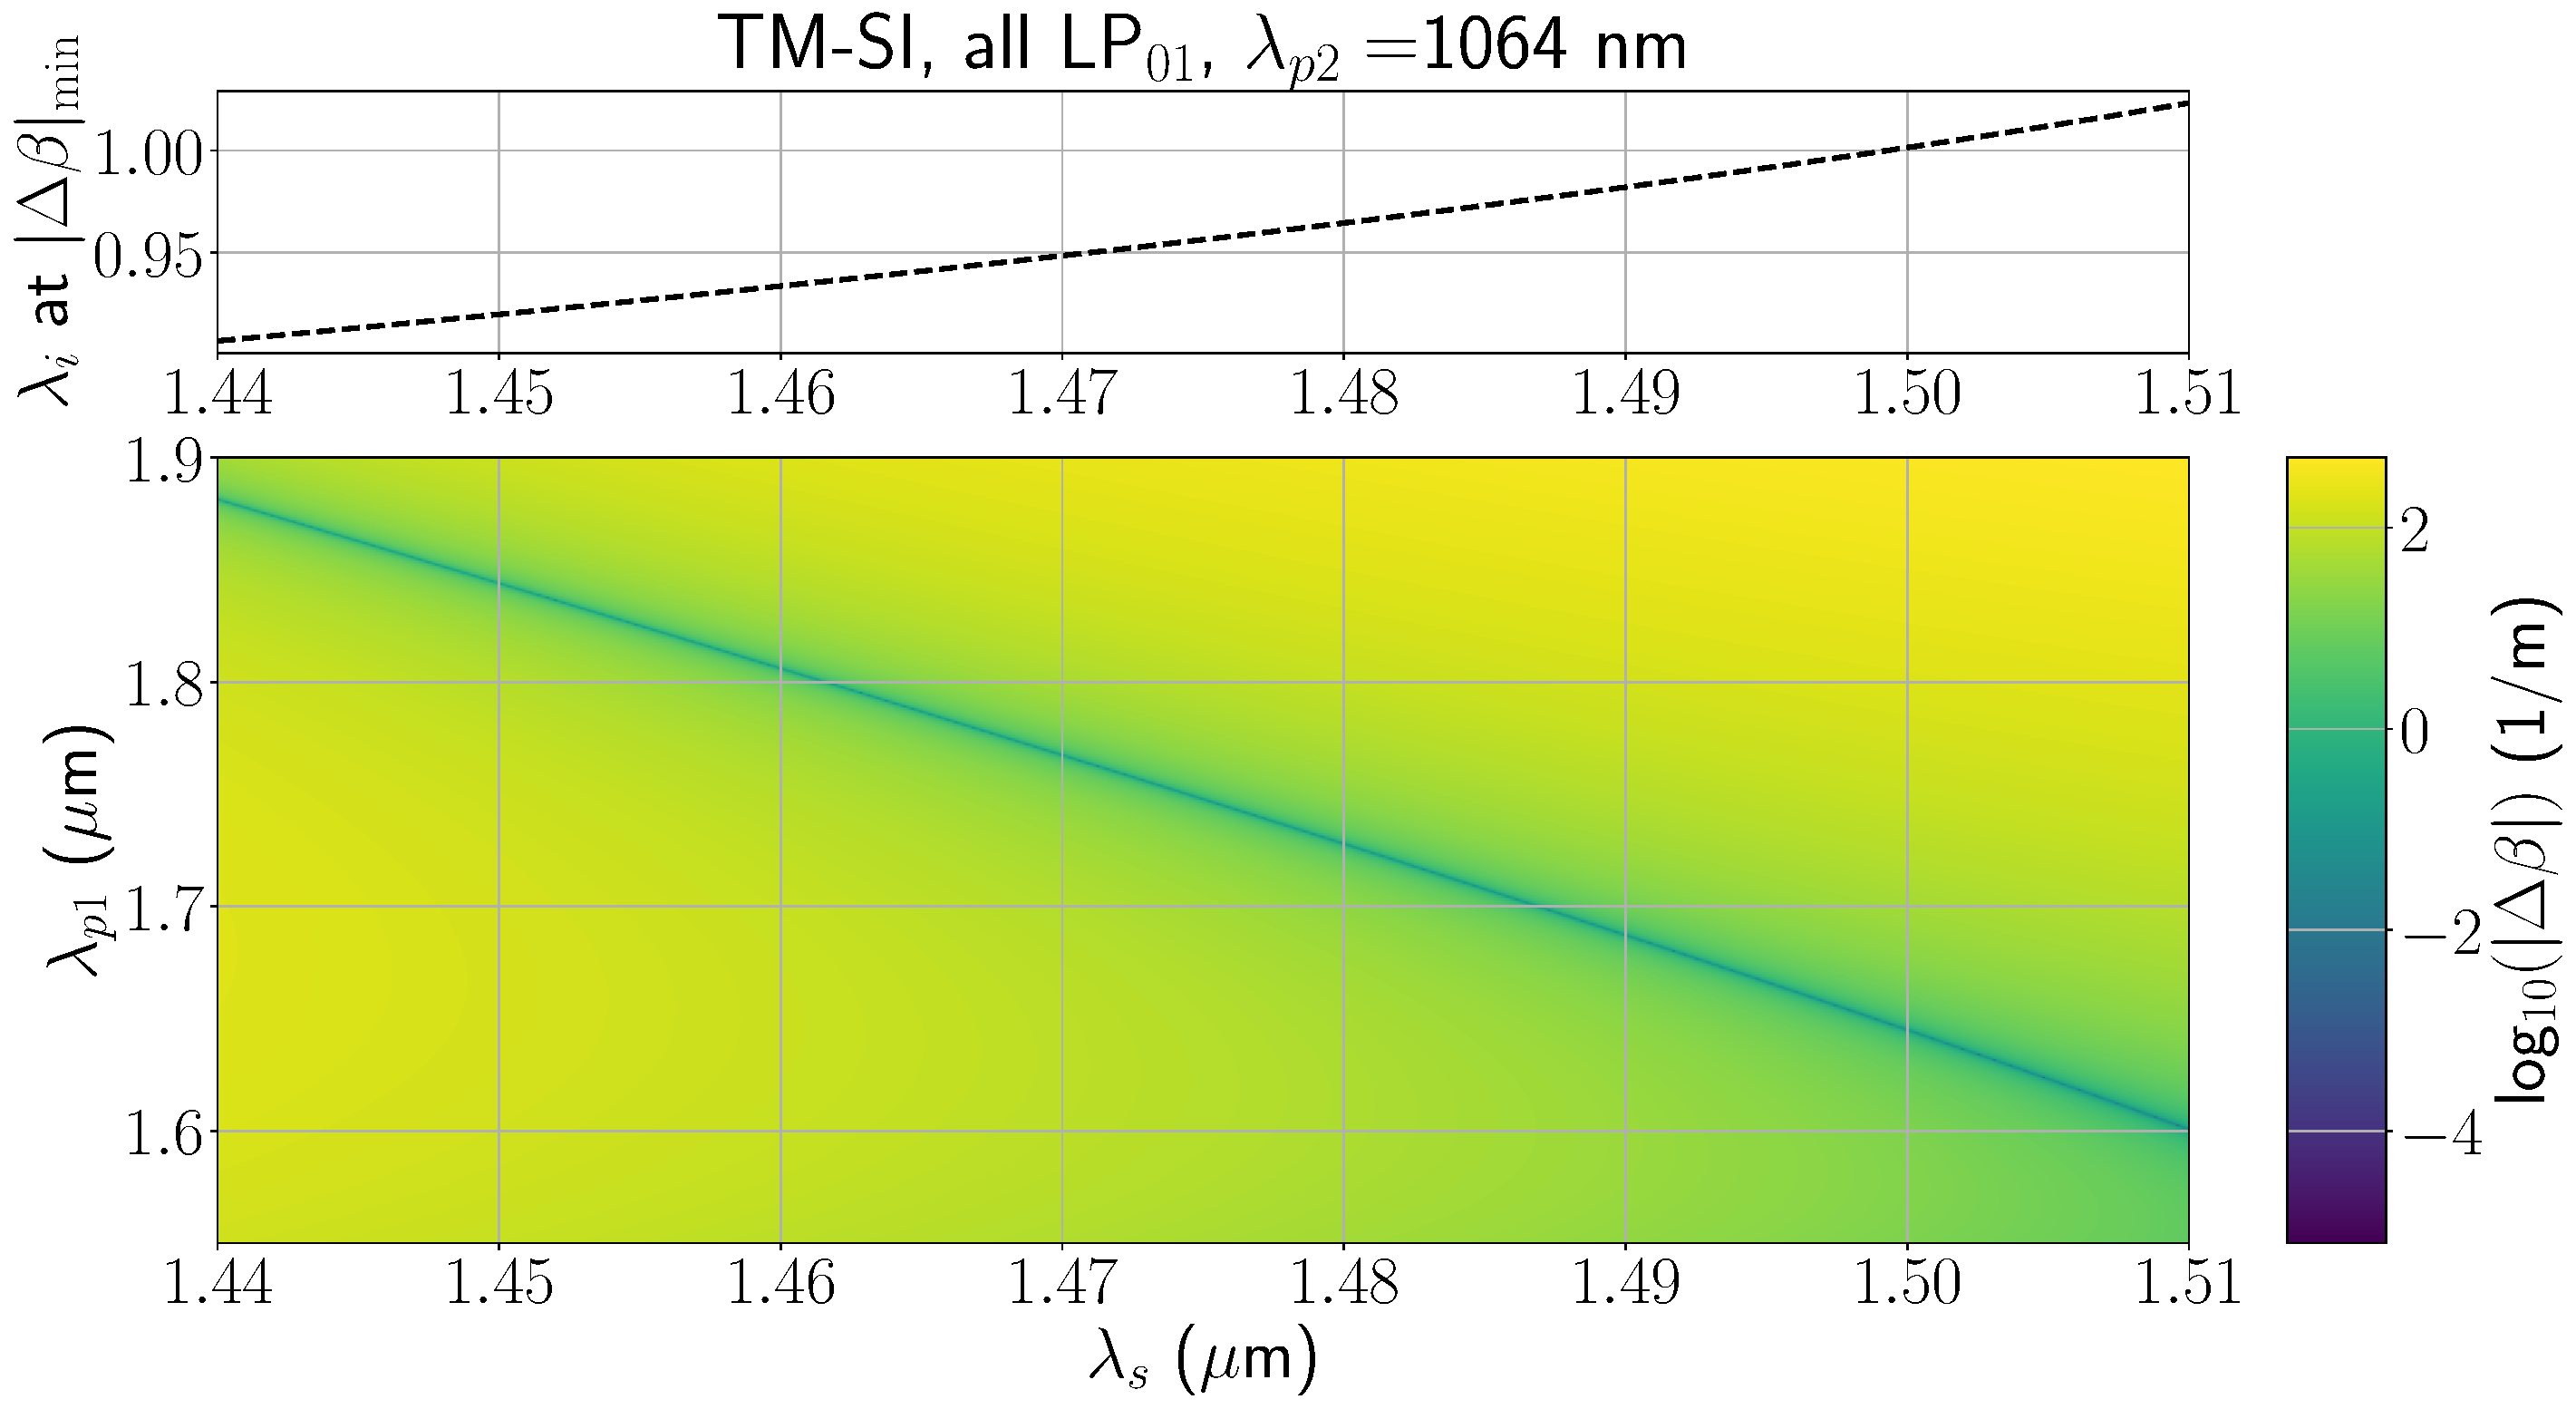
\includegraphics[width=0.8\textwidth]{./figs/TMSI_all_LP01_1064_2d_dbeta.pdf}
    \caption{}
    \label{fig:fmf_1064}
\end{figure}
\end{document}
